\section{Results}
\label{sec:results}

\subsection{The QNN learns the task, and a classical network of similar size does slightly better}
\label{sec:res-mnist}

\begin{table}[t]
\centering
\caption{Test accuracy on $4\times4$ binarised MNIST 3-vs-6 (mean $\pm$ std over \valMnistSeeds{} seeds,
\valMnistNTrain{} training and \valMnistNTest{} test images per seed, \valMnistEpochs{} epochs). A
lookup table over training patterns reaches \valCeilFour{}. Training time is the mean wall-clock time
of simulated training on CPU. It varied by up to $3\times$ across seeds with machine load.}
\label{tab:mnist}
\begin{tabular}{lrrr}
\toprule
Model & Parameters & Test accuracy & Train time (s) \\
\midrule
QNN (quantum readout) & 32 & 0.868 $\pm$ 0.023 & 543 \\
QNN + dense head (hybrid) & 185 & 0.906 $\pm$ 0.006 & 636 \\
classical MLP & 37 & \textbf{0.909 $\pm$ 0.006} & 5 \\
\bottomrule
\end{tabular}

\end{table}

\begin{figure}[t]
\centering
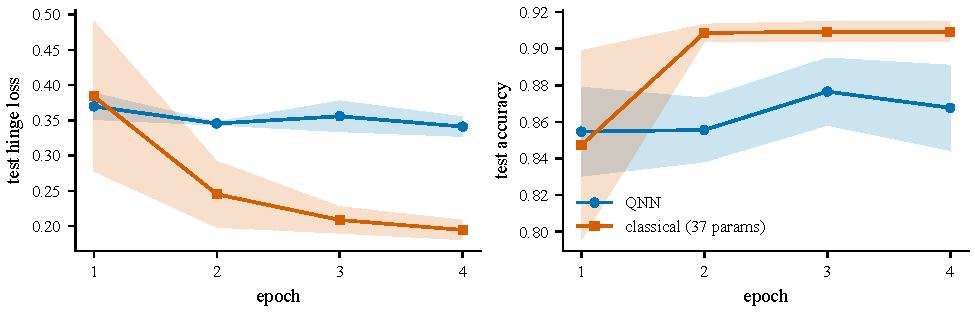
\includegraphics[width=\linewidth]{figures/mnist_qnn.pdf}
\caption{The classical network overtakes the QNN after the first epoch and ends higher, with less spread across seeds.
Test hinge loss and accuracy per epoch, mean $\pm$ std over \valMnistSeeds{} seeds.}
\label{fig:mnist}
\end{figure}

The QNN reaches \valQnnAcc{} $\pm$ \valQnnStd{} test accuracy (Table~\ref{tab:mnist},
Fig.~\ref{fig:mnist}). The classical network, with \valClassicalParams{} parameters against the QNN's
\valQnnParams{}, reaches \valClassicalAcc{} $\pm$ \valClassicalStd{}. Both are bounded by the input:
binarising to $4\times4$ leaves \valPatternsFour{} distinct training patterns, and predicting each
pattern's majority label scores \valCeilFour{} on the full test set. The classical model sits almost on
that ceiling, so on this input there is little room for any model to do better. The QNN also took about
\valQnnSecs{}\,s to train in simulation, against \valClassicalSecs{}\,s for the classical network.

\subsection{A classical head on the readouts closes the gap}
\label{sec:res-hybrid}

\begin{figure}[t]
\centering
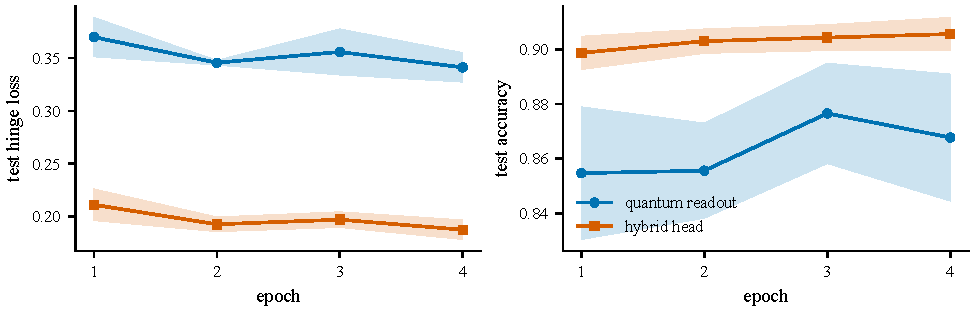
\includegraphics[width=\linewidth]{figures/hybrid.pdf}
\caption{Reading out every qubit and adding a small dense head improves accuracy and reduces
variance across seeds. Same data, seeds and circuit as Fig.~\ref{fig:mnist}.}
\label{fig:hybrid}
\end{figure}

Measuring $\langle Z\rangle$ on all 17 qubits and passing the values through an 8-unit dense layer raises
accuracy by \valHybridGain{} points, to \valHybridAcc{} $\pm$ \valHybridStd{} (Fig.~\ref{fig:hybrid}).
This matches the classical model. The gain cannot be attributed to the circuit alone: the hybrid model
has \valHybridParams{} parameters, most of them classical, and 16 of its 17 readouts are on data qubits, which
start in the input's basis state.

\subsection{Gradients shrink as random circuits grow}
\label{sec:res-barren}

\begin{figure}[t]
\centering
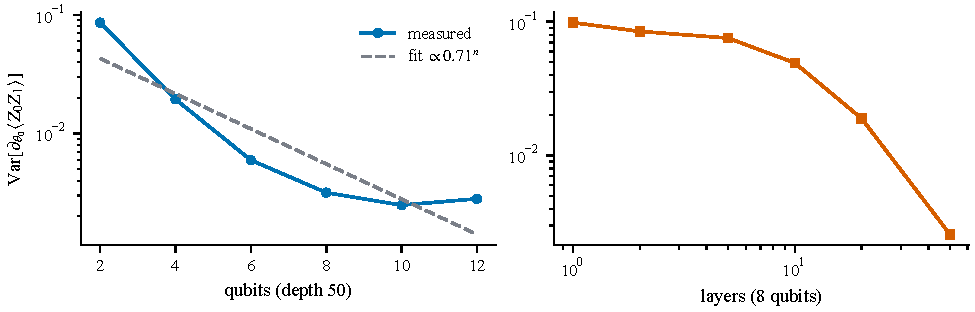
\includegraphics[width=\linewidth]{figures/barren_plateaus.pdf}
\caption{Gradient variance falls with width and with depth. Left: variance of
$\partial\langle Z_0Z_1\rangle/\partial\theta_0$ against qubit count at \valBpFixedDepth{} layers, with a
log-linear fit over all points. Right: against depth at \valBpFixedQubits{} qubits. Each point uses
\valBpCircuits{} random circuits.}
\label{fig:barren}
\end{figure}

At \valBpFixedDepth{} layers, the gradient variance falls from \valBpVarMinQ{} at \valBpMinQ{} qubits to
\valBpVarEight{} at 8 qubits, a factor of \valBpRatioEight{} (Fig.~\ref{fig:barren}, left). Beyond 8
qubits it stops falling in our sweep, reaching \valBpVarMaxQ{} at \valBpMaxQ{} qubits, so a single
exponential (decay factor \valBpDecay{} per qubit) describes the trend only loosely. The depth sweep
suggests why. At \valBpFixedQubits{} qubits the variance is still falling at \valBpMaxDepth{} layers,
\valBpDepthRatio{} times below its single-layer value (Fig.~\ref{fig:barren}, right), so
\valBpFixedDepth{} layers are probably not enough for the wider circuits to behave as random as the
theory assumes \citep{mcclean2018barren}. We did not test this directly.

\subsection{Depolarizing noise erodes accuracy quickly}
\label{sec:res-noise}

\begin{figure}[t]
\centering
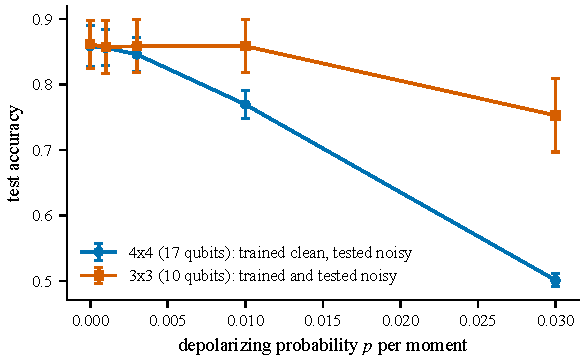
\includegraphics[width=0.6\linewidth]{figures/noise.pdf}
\caption{Trained $4\times4$ QNNs fall to chance by $p=\valNoiseMaxP$. Smaller $3\times3$ models
trained with the noise present hold their accuracy up to $p=0.01$. The two curves are different
models with different circuit depths, so compare slopes, not heights. Mean $\pm$ std over
\valNoiseSeeds{} seeds; \valNoiseReps{} trajectories per expectation.}
\label{fig:noise}
\end{figure}

\begin{table}[t]
\centering
\caption{Test accuracy under depolarizing noise with probability $p$ per qubit per moment (mean $\pm$ std over
\valNoiseSeeds{} seeds).}
\label{tab:noise}
\begin{tabular}{lcc}
\toprule
$p$ & 3$\times$3, trained with noise & 4$\times$4, trained clean, tested with noise \\
\midrule
0.0 & 0.862 $\pm$ 0.036 & 0.859 $\pm$ 0.031 \\
0.001 & 0.857 $\pm$ 0.040 & 0.856 $\pm$ 0.028 \\
0.003 & 0.859 $\pm$ 0.040 & 0.846 $\pm$ 0.026 \\
0.01 & 0.859 $\pm$ 0.040 & 0.770 $\pm$ 0.022 \\
0.03 & 0.753 $\pm$ 0.056 & 0.501 $\pm$ 0.010 \\
\bottomrule
\end{tabular}

\end{table}

The $4\times4$ QNNs from \S\ref{sec:res-mnist}, tested under noise, go from \valNoiseEvClean{} without
noise to \valNoiseEvMid{} at $p=0.01$ and \valNoiseEvMax{} at $p=\valNoiseMaxP$, which is chance
(Fig.~\ref{fig:noise}, Table~\ref{tab:noise}). The channel acts after every moment of a circuit with 32
two-qubit couplings, so errors accumulate before the readout is measured. The $3\times3$ models trained with the noise
present keep \valNoiseTrMid{} at $p=0.01$, against \valNoiseTrClean{} without noise, and drop to
\valNoiseTrMax{} at $p=\valNoiseMaxP$. This comparison is confounded: the $3\times3$ circuit has 18
couplings rather than 32, so it accumulates less noise whether or not it is trained with it. Separating
the effect of noise-aware training from circuit size would need noisy training at $4\times4$, which was
too slow for us (\S\ref{sec:setup}).
